\section{Simulation Analysis}
\label{sec:simulation} 

\par In these section we represent the plots that were produced by doing operating point using Ngspice. These plots represents the Voltage on Envelope Detector and the output voltage of the circuit.


\begin{figure} [!htb] 
  \minipage{0.9\textwidth}
  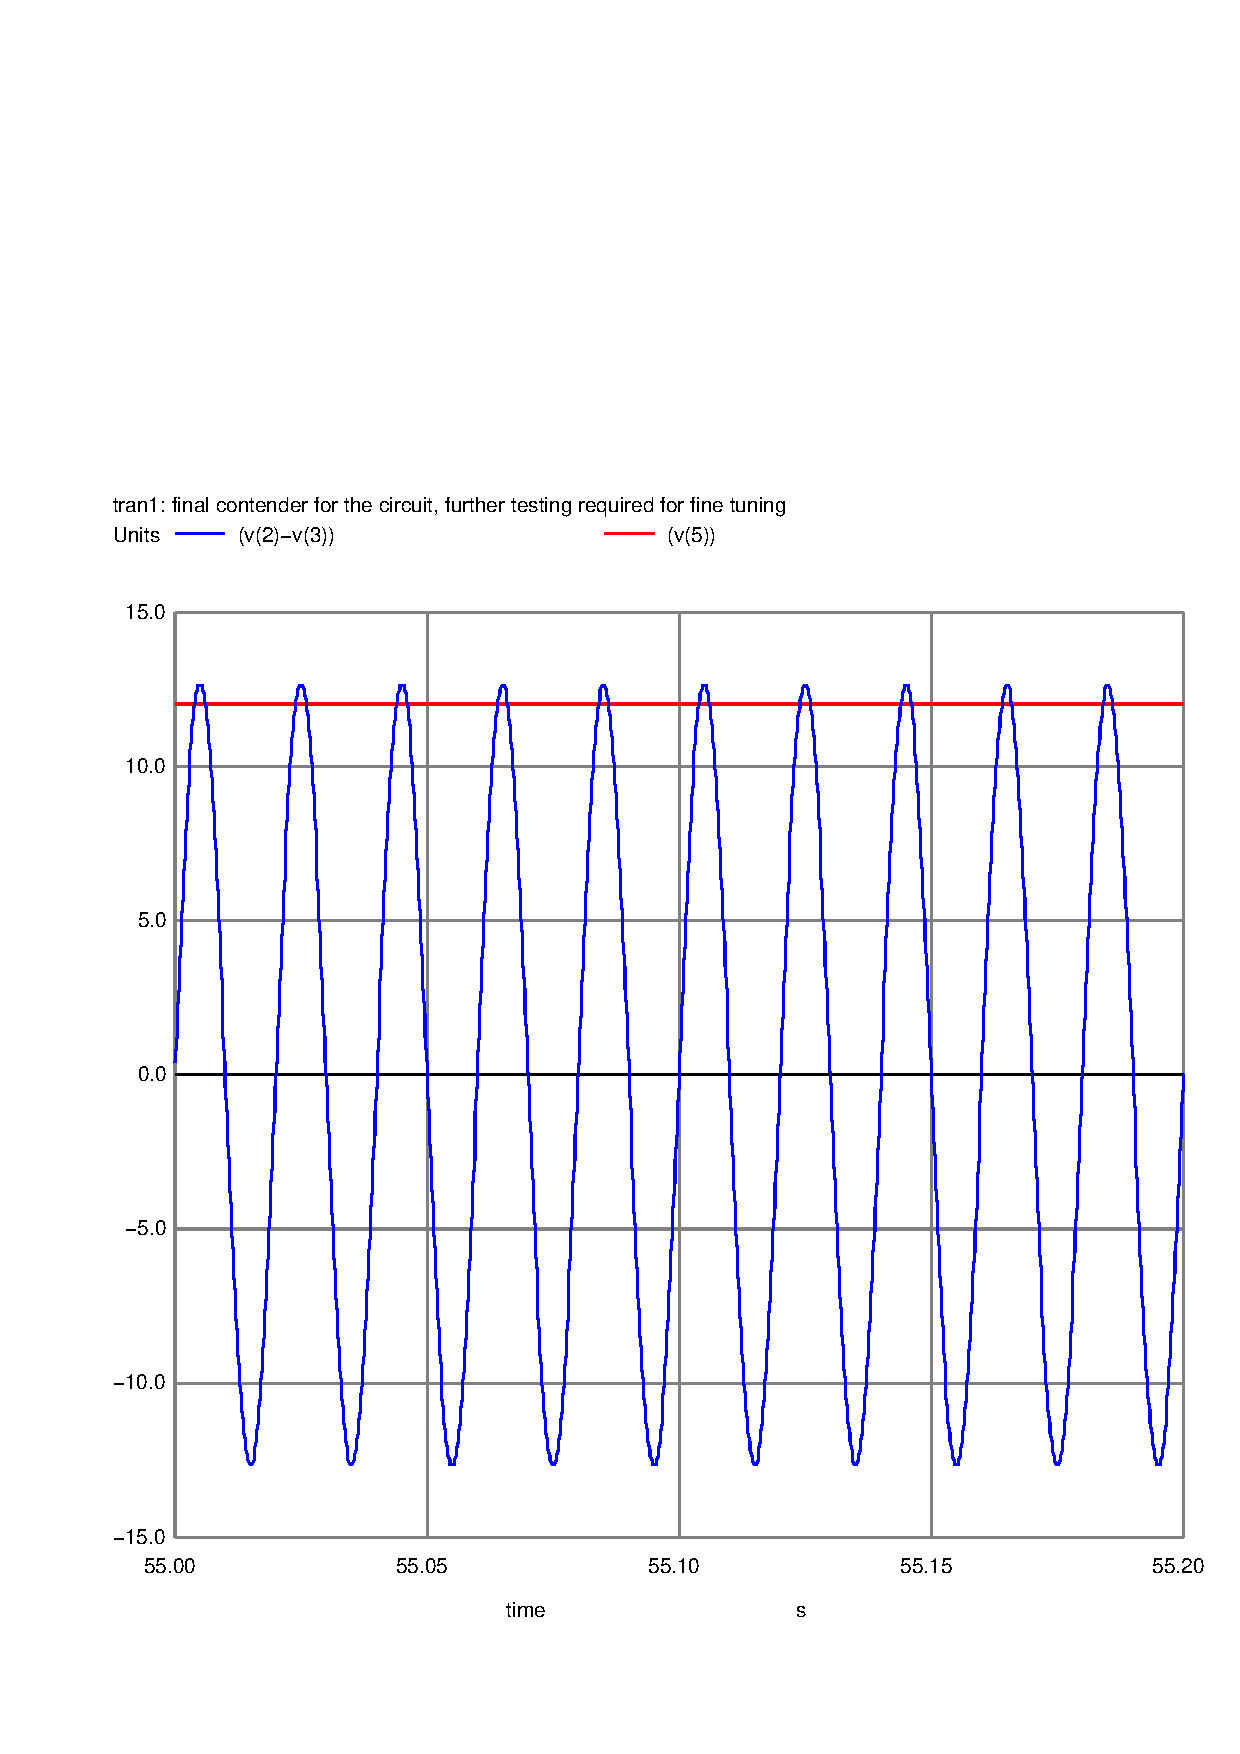
\includegraphics[width=\linewidth]{out.pdf}
  \caption{Envelope Detector and Output Voltages}
  \label{fig:theoplots}
  \endminipage\hfill
\end{figure}



\begin{figure} [!htb]
  \minipage{0.9\textwidth}
  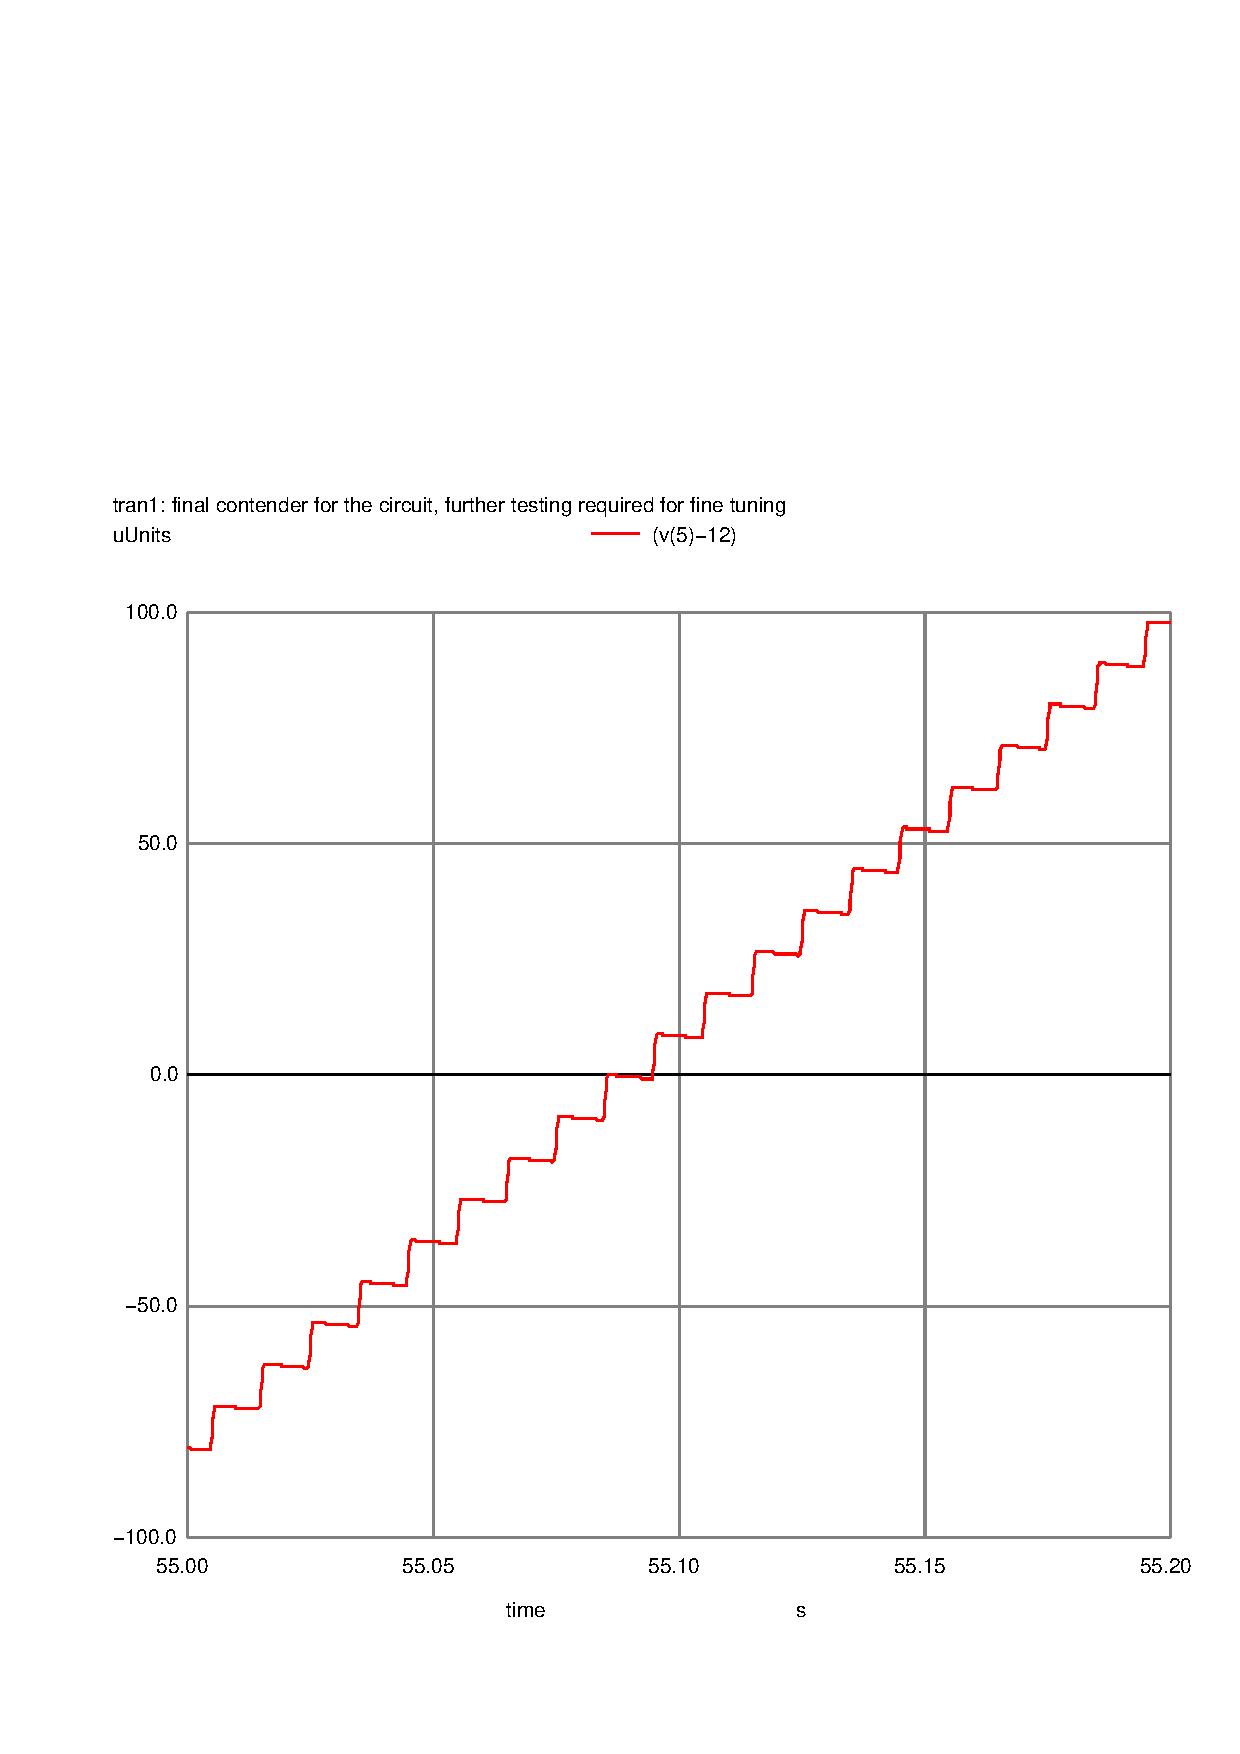
\includegraphics[width=\linewidth]{zoom.pdf}
  \caption{Output AC component + DC deviation}
  \label{fig:theoplots}
  \endminipage\hfill
\end{figure}


\par And finally to conclute the requirements for the simulation analysis, we have computed the results of the voltage ripple and the output DC level.  

\FloatBarrier
\begin{table}[h]
  \centering
  \begin{tabular}{|c|c|c|}
    \hline    
    maximum(v(5)) & 1.200010e+01\\ \hline
minimum(v(5)) & 1.199992e+01\\ \hline
mean(v(5)) & 1.200001e+01\\ \hline

    \hline
  \end{tabular}
  \caption{Ripple an DC voltages}
  \label{tab:Octave}
\end{table}
\FloatBarrier  

From this table we can remove the ripple voltage value, that match with the difference: $V_{ripple}=maximum(v(5))-minimum(v(5))$, which in this case has a value of $V_{ripple}=1.8e-04$. And also the value of the DC level, which in this case is represented by the variable $mean(v(5))$


%colocar valores
% não consigo encontrar os valores certos para colocar aqui, nomeadamente os do ripple e do DC level, helppp
